\chapter{Interpretability-performance trade-offs}\label{sec:exps2}
In this chapter, we study the interpretability-performance trade-offs of different policies.
For each environment considered we experiment with the best in class policies obtained in the previous chapter.  
For each environment we hence study five decision tree policies with varying number of nodes, five oblique decision tree policies with varying number of nodes, one linear policy, and four relu neural network policies with varying number of hidden units (cf. table~\ref{tab:policy-classes}).
To obtain fair interpretability measurements, in our case inference speeds in seconds or sizes in bytes (cf. Sec~\ref{sec:unfold}), we run each unfolded policy \textbf{on the same dedicated CPU} for 100 new environment episodes.
Since all the policies process computations roughly the same way, and since they are executed on the exact same device in the same conditions we believe the results presented next are a good illustration of our methodology (cf. section~\ref{sec:unfold}) 
can be used for interpretability research.
\section{Is it possible to compute interpretable policies for high-dimensional environments?}

\begin{figure}
    \centering
    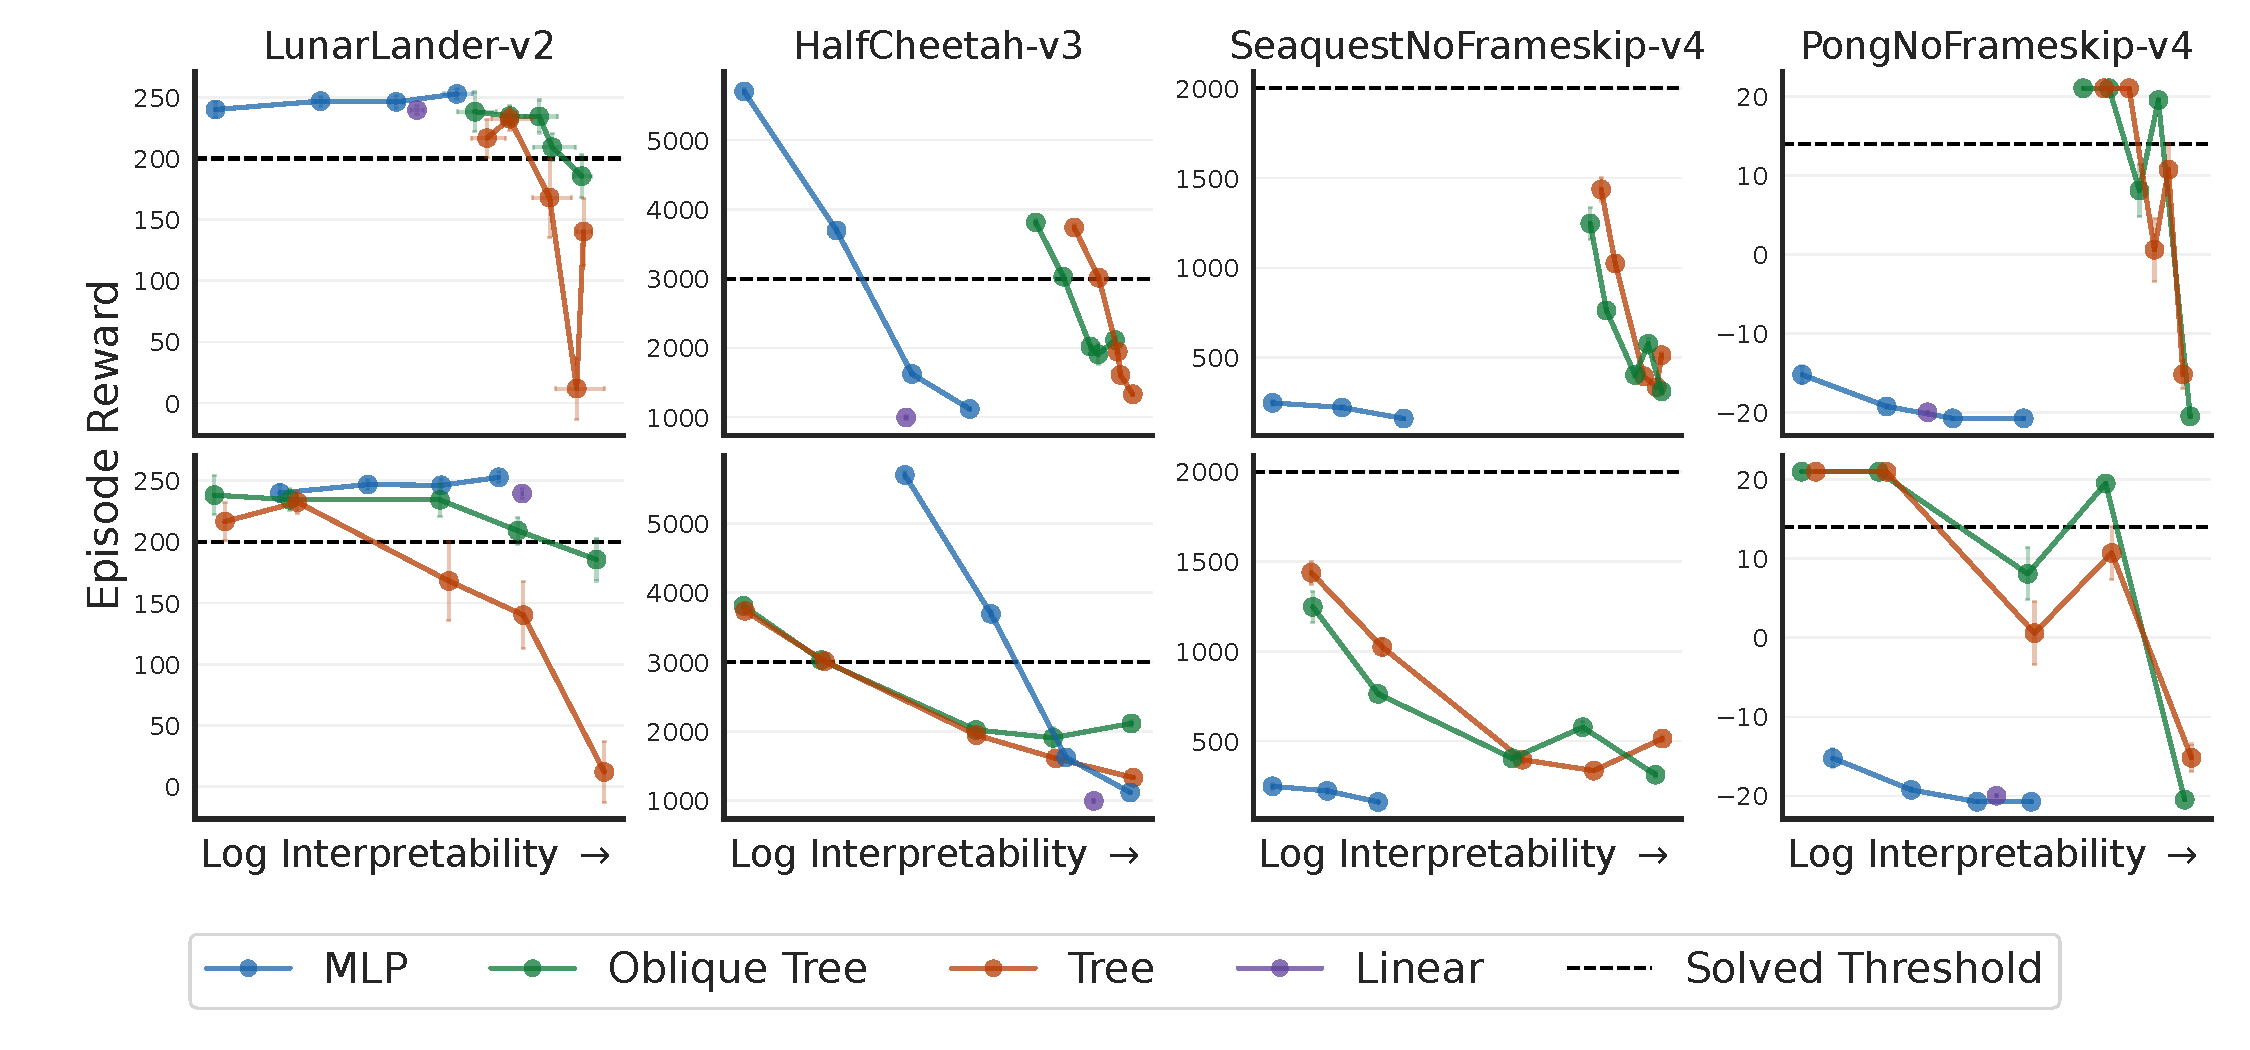
\includegraphics[trim={1.4cm 0 0 0},clip,width=1\textwidth]{images/images_part3/trade_off_select_combine_one_plot.pdf}
    \caption{interpretability-Performance trade-offs. Top row, interpretability is measured with step inference times. Bottom row, the interpretability is measured with policy size. We plot 95\% bootstrapped confidence intervals around means on both axes.}
    \label{fig:trade-off-summary}
\end{figure}
% \begin{figure}
%     \centering
%     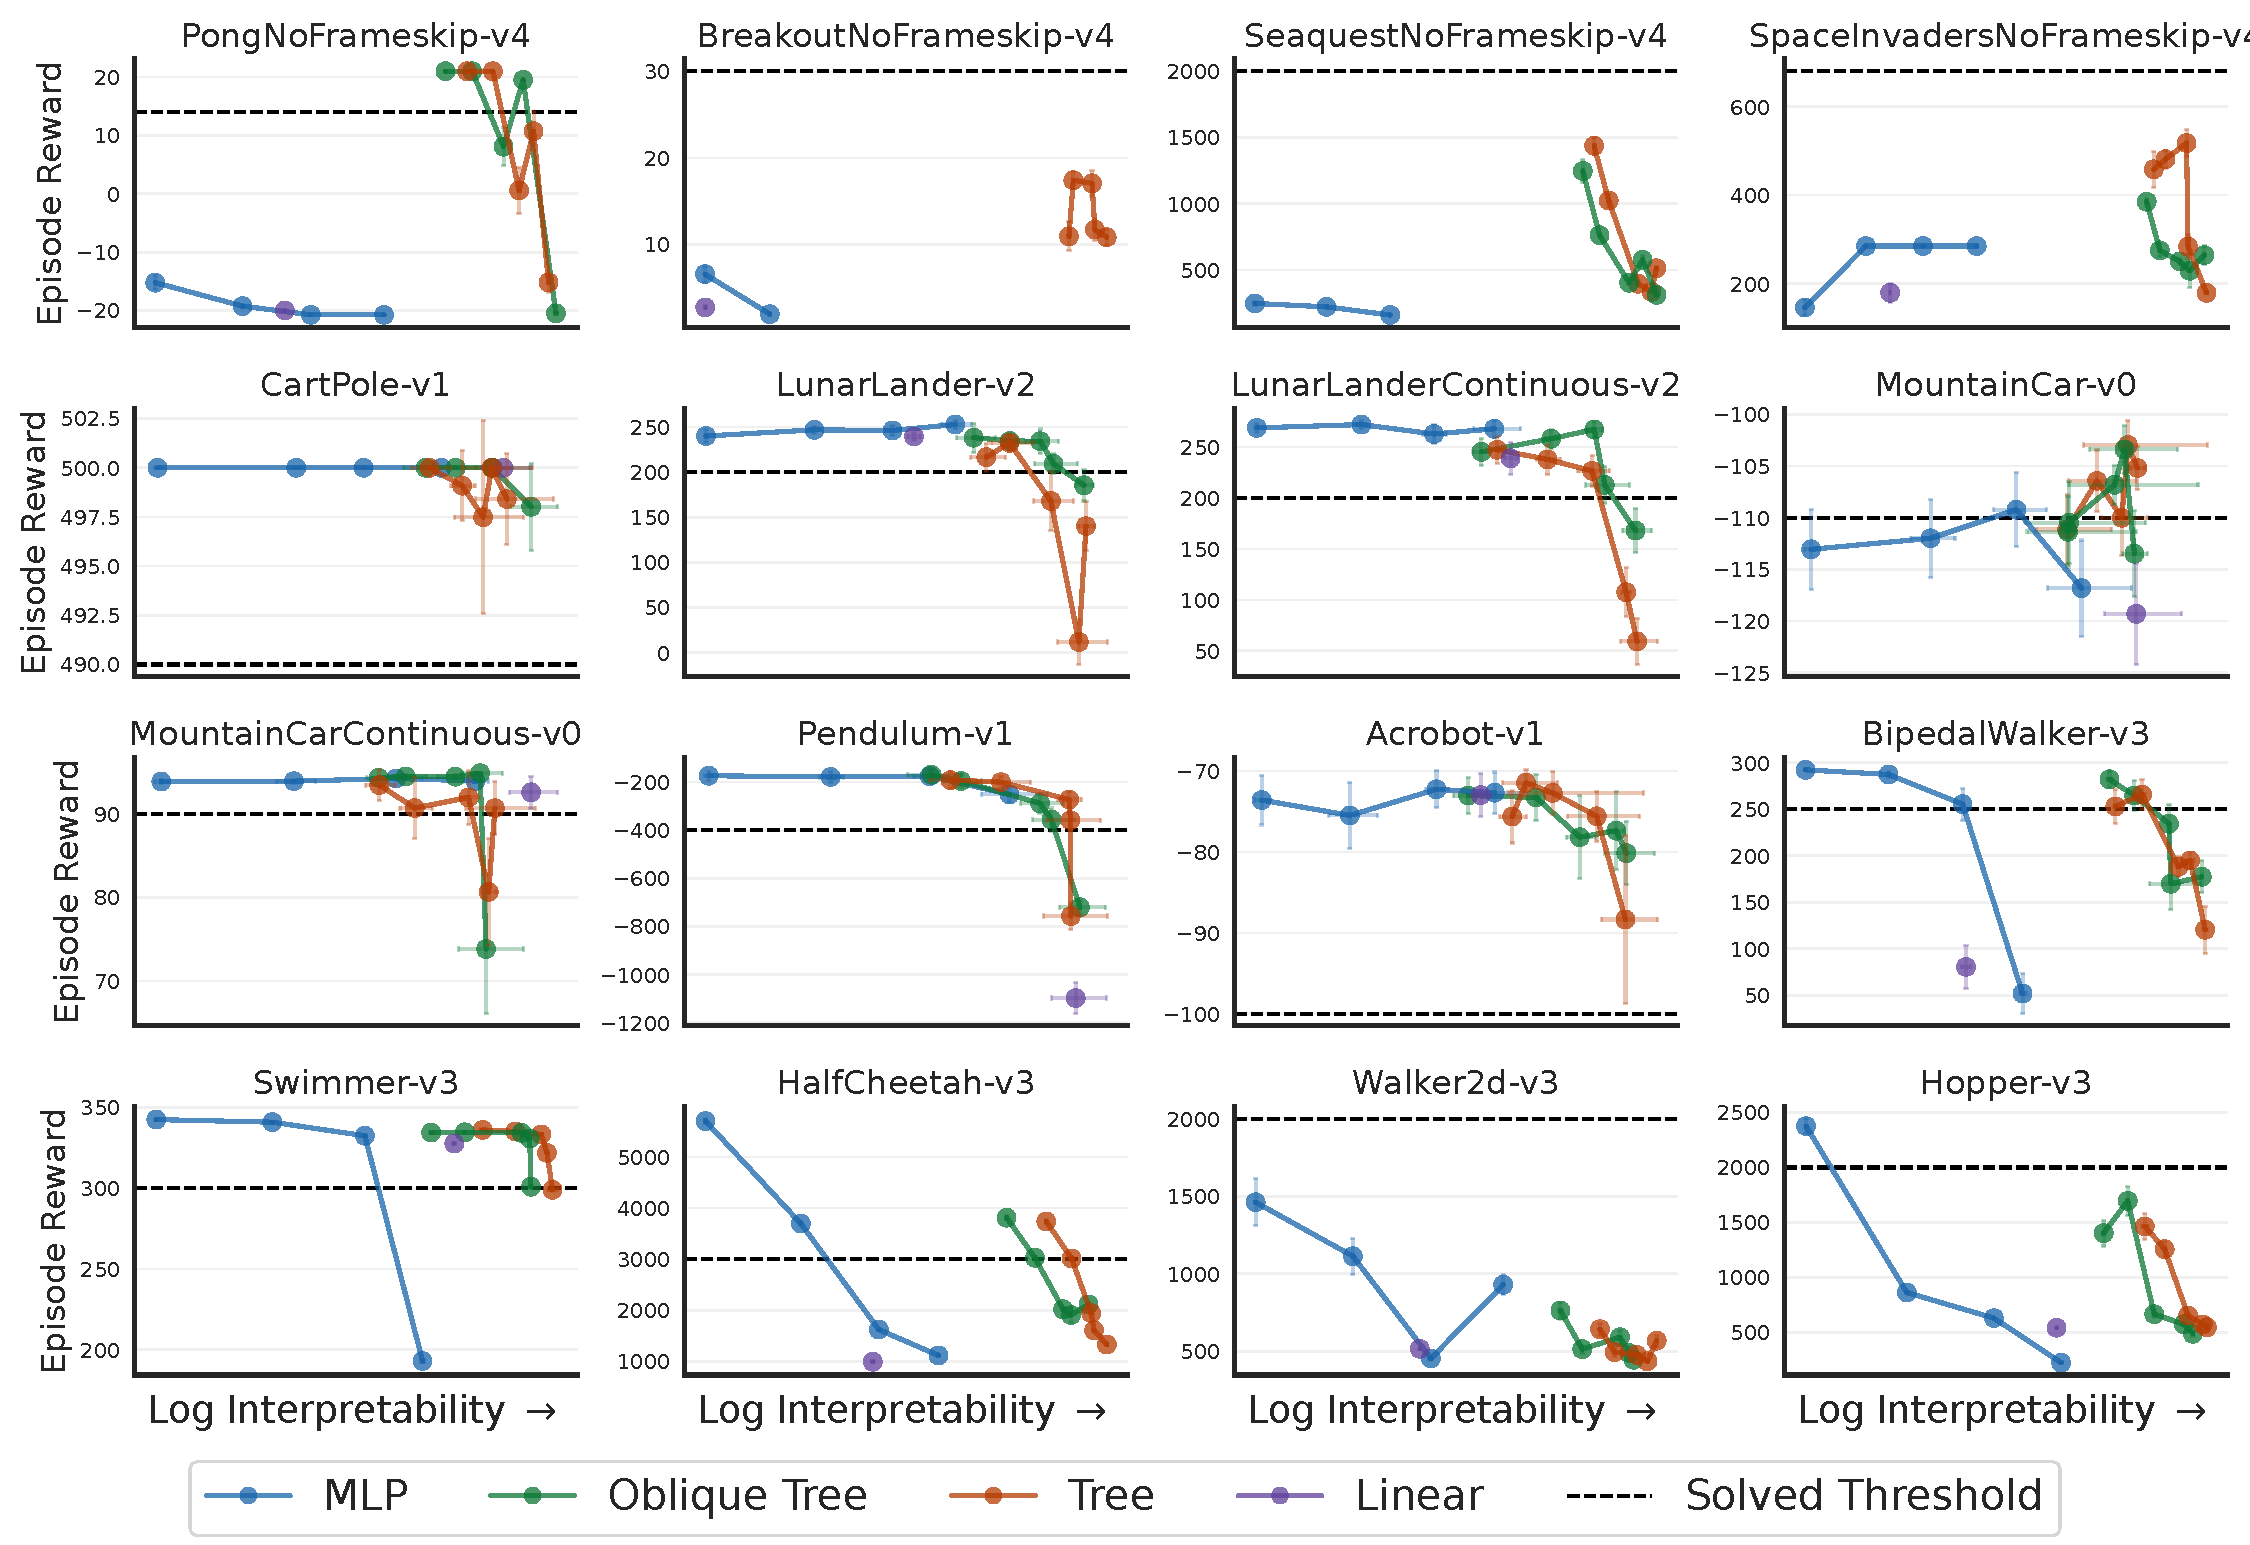
\includegraphics[width=1\linewidth]{images/images_part3/trade_off_step_times.pdf}
%     \caption{Trade-off Cumulative Reward vs. Step Inference Time. We plot 95\% bootstrapped confidence intervals around means on both axes.}
%     \label{fig:trade-off-summary}
% \end{figure}

In figure~\ref{fig:trade-off-summary}, we present results only for part of the environments that we believe are the most representative.
This allows us to have a compact comparison of policy trade-offs with either of the metrics from section~\ref{sec:unfold}.
The full trade-offs are presented in appendix~\ref{sec:trade-offs-full}.
In \cite{glanois-survey}, authors claim that computing an interpretable policy for high-dimensional MDPs, i.e. environments where the number of state features is high, is difficult since it is similar to program synthesis which is known to be NP-hard \cite{program-synth}.
Using our measures of interpretability, we can corroborate this claim.
On figure \ref{fig:trade-off-summary}, we can indeed observe that some relatively interpretable policies can solve object-centric Pong (20 state features) or HalfCheetah (17 state features). 
For example, the oblique tree policy from figure~\ref{lst:pong}, represented by the second right most green dot on figure~\ref{fig:trade-off-summary}, is among the most interpretable policies for Pong w.r.t to both policy size and policy inference time, and has RL objective value (cf. definition~\ref{def:mdp-obj}) above the solving threshold.  
However, for very high-dimensional environments like Seaquest (180 state features), none of our policies, even the less interpretable ones (relu networks with two hidden layer units of size sixteen), can solve the game.
This observation resonates with the first part of the manuscript where we showed that even in controlled experiments where an interpretable policy is optimal, no RL algorithm to retrieve it.
This yields the following question.

\section{For what environment are there good interpretable policies?}
We fitted a random forest regressor~\cite{random} to predict the interpretability values of our best in class policies using environment attributes. 
In table~\ref{tab:combined_importance}, we report the importance of each environment attribute when it comes to accurately predicting interpretability scores.
We show that as hinted previously, the number of state features of the environment is determining to predict the interpretability of good policies.
Unsurprisingly, expert attributes also influence interpretability: for the environments where there is a positive large gap between expert and threshold rewards, the task could be considered easy and vice-versa.

\begin{table}
\centering
\small
\begin{tabular}{lcc}
\toprule
Environment Attributes & Importance for Step inference & Importance for Policy size \\
\midrule
State features & \textbf{80.87} & \textbf{35.52} \\
Expert episodes lengths & 11.39 & 9.28 \\
Episode reward of random & 2.26 & 4.75 \\
Expert episode reward & 1.51 & 16.80 \\
Episode reward to solve & 1.41 & 14.26 \\
Actions dimension & 1.41 & 2.02 \\
Expert reward - Solve reward & 1.15 & 17.37 \\
\bottomrule
\end{tabular}
\caption{Environment attributes importance to predict interpretability of the best in class policies obtained in chapter~\ref{sec:exps1}.}
\label{tab:combined_importance}
\end{table}

\section{How does interpretability influence performance?}
In \cite{empirical-evidence,theory1}, authors show the existence of linear and tree policies respectively that solve MuJoCo and continuous maze environments respectively.
This means that there exist environments for which policies more interpretable than deep neural networks can still compete performance-wise.
Our evaluation indeed shows the existence of such environments.
On figure~\ref{fig:trade-off-summary} we observe that on, e.g., LunarLander, increasing policy interpretability up to a certain point does not decrease reward.
For example, for neural networks, all the the blue dots, both for the policy size and policy inference time metrics, are above the solving thresholds, which means that relu networks with two hidden layers of two units each perform as well as a relu network with two hidden layers of sixteen units each. 
Surprisingly, we can observe that for Pong a minimum level of interpretability is required to solve the game.
Indeed, as stated in \cite{study-0}, optimizing interpretability can also be seen as regularizing the policy which can increase generalization capabilities. 
The key observation is that the policy class achieving the best interpretability-performance trade-off depends on the problem.
Indeed, independent of the interpretability metric, we see on figure~\ref{fig:trade-off-summary} that for LunarLander it is a neural network that achieves the best trade-off while for Pong it is a tree.
This means that, when research interpretability one needs to be extra careful when using model interpretability assumptions presented in e.g. figure~\ref{fig:interpretability-performance-tradeoff}.
Next, we compare our proxies for interpretability with another one; the verification time of policies used in \cite{viper,lens-complexity}.


\section{Verifying interpretable policies}\label{sec:verif}
\cite{lens-complexity} states that the cost of formally verifying properties of a relu neural network scales exponentially with the number of parameters (hidden units).
Hence, they propose to measure interpretability of a policy as the computations required to verify properties of actions given state features subspaces, what they call local explainability queries \cite{query}.
Interestingly, VIPER (algorithm~\ref{alg:viper},~\cite{viper}) was designed in hope to get policies tht were easy to verify.
In practice, this amounts to passing a subspace of state features and a subspace of (continuous) action features and solving the SAT problem of finding at least one state in the subspace for which the policy outputs an action in the action subspace.
For example, for the LunarLander problem, a verification query could be to verify if when the y-position of the lander is below some threshold value, i.e, when the lander is close to the ground, there exists a state such that the tested policy would output the action of pushing towards the ground: if the solver returns \texttt{True}, then there is a risk that the lander crashes when deployed because it might push towards the ground even at low altitude.

Designing interesting queries covering all risks is an open problem, hence to evaluate the verification times of our best in class policies, we generate 500 random queries per environment by sampling state and action subspaces uniformly.
Out of those queries we only report the verification times of UNSAT queries since to verify that, e.g., the lander does not crash we want the example query mentioned above to be UNSAT.
We also only verify instances of neural networks and linear policies using the solver~\cite{maraboupy} for this experiment as verifying decision trees requires a different software~\cite{z3} for which verification times would not be comparable.
We verify each policy using the same verification algorithm with the same hyperparameters and queries on the same CPU to obtain faire measurements of verification times.
We leave it to future work to write decision tree policies as relu networks to then compare their verification times fairly.
Indeed it is known that oblique decision trees can be written as a relu neural networks~\cite{Lee2020Oblique}.

\begin{figure}[ht]
    \centering
    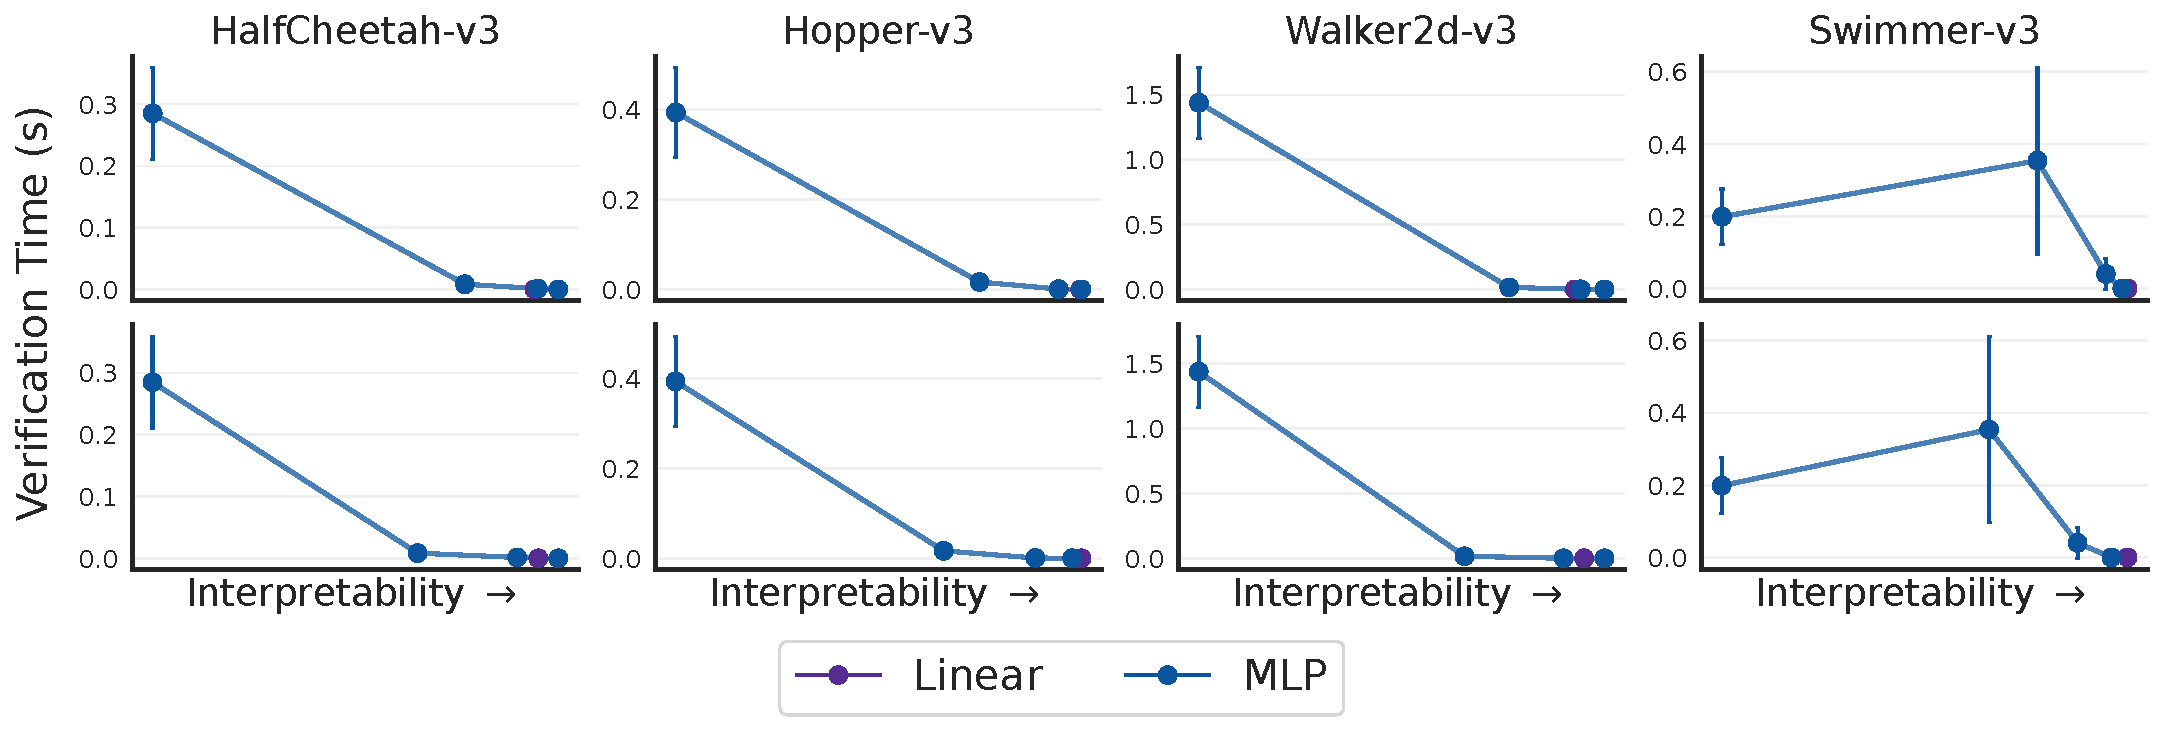
\includegraphics[width=1\linewidth]{images/images_part3/verification_tradeoff.pdf}
    \caption{Verification time as a function of policy interpretability. Top row, interpretability is measured with step inference times. Bottom row, the interpretability is measured with policy size. We plot 95\% confidence intervals around means on both axes.}
    \label{fig:trade-off-verif}
\end{figure}

On figure \ref{fig:trade-off-verif}, we can observe that verification time decreases exponentially with our measures of interpretability as shown theoretically in \cite{lens-complexity}.
This is another good validation of our proposed methodology as well as a motivation to learn interpretable policies. 

\section{Limitations and conclusions}\label{sec:ccl-imit}
In this part of the manuscript, we have proposed to write policies for MDPs from different model classes in a unified language.
We believe that unfolding policies (cf. section~\ref{sec:unfold}) allows for fair measurements of interpretability proxies.
In particular, we unfolded thousands of policies from different model classes (cf. table~\ref{tab:policy-classes}), and showed that comparing inference speed and sizes gave conclusions about interpretability similar to existing user studies (cf. section~\ref{sec:exps1}).

Using the proposed methodology, we were able to illustrate the trade-offs between the RL objective (cf. definition~\ref{def:mdp-obj}) at the core of this manuscript and interpretability of policies.
We showed the crucial need of careful methodology as different different policy classes yield different trade-offs on different environment: decision trees are not always more interpretable than neural networks. 

A nice property of our methodology is that it is independent of the learning algorithm of the interpretable policy.
We chose imitation learning but it could have been a random search in the policies parameters space \cite{empirical-evidence}.

Furthermore, there should be no limitation to use our methodology to evaluate the interpretability of arbitrary compositions of linear policies, trees and oblique trees, and neural networks, such as the hybrid policies from \cite{shindo2024blendrl}.

Even though using episodic inference does not change the trade-offs compared to step inference time (cf. appendix~\ref{fig:trade-off} and~\ref{fig:trade-off-episode}), it is important to discuss this nuance in future work since a key difference between supervised learning and reinforcement learning interpretability could be that human operators would read policies multiple times until the end of a decision process.
Using episodic metrics for interpretability is not as straightforward as someone would think as for some MDPs, e.g. Acrobot, the episodes lengths depend on the policy.

We also did not evaluate the role of sparsity in the interpretability of linear and neural network policies even thought this could greatly influence the inference time.
For completeness, when unfolding policies, we should delete operations including near-zero parameters. 
In the future we should also evaluate the influences of different unfolding procedures.
For example, the number of significant digits in the values of parameters might affect the measures of interpretability.

Most importantly, we should further validate our methodology with user studies of the unfolded policies we open sourced\footnote{\url{https://github.com/KohlerHECTOR/interpretable-rl-zoo}}.

We hope that our methodology as well as the provided baselines will pave the way to a more rigorous science of interpretable reinforcement learning.
